\section{L'API de l'UAV}
\subsection{Choix du drone}

Maintenant que nous avons un environnement de simulation qui fonctionne nous souhaiterions 
obtenir des résultats sur des UAV réels. 

Le DJI Matrix 600 est la plateforme idéale pour développer. On peut embarquer un
ordinateur (Raspberry Pi, NVIDIA Jetson). Une API interfaçable avec ROS permet de
piloter l’UAV en se limitant aux algorithmes haut-niveaux. De plus, il existe un modèle
Gazebo pour valider et entraîner nos algorithmes en simulation avant de les embarquer.
Cependant, ce drone est grand (1.5 m x 1.5 m x 1 m) donc puissant, il faut donc un
environnement de test dimensionné et adapté à son utilisation. Des tests à l’ENSTA
Bretagne ne sont pas envisageables, nous avons donc opté pour un autre UAV. 

\begin{figure}[!htb]
    \centering
    \begin{subfigure}[b]{0.4\textwidth}
        \centering
        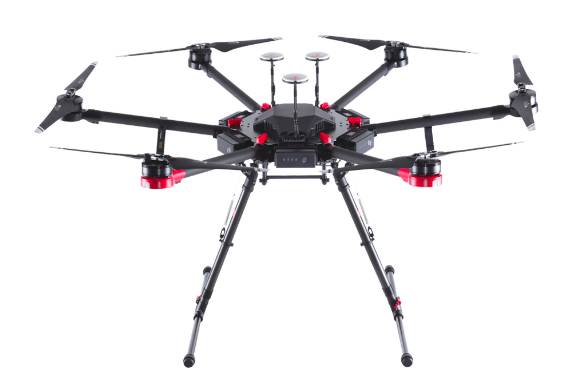
\includegraphics[width=\textwidth]{./api/matrix.png}
        \caption{DJI Matrix 600}
        \label{fig:marker}
    \end{subfigure}
    \hfill
    \begin{subfigure}[b]{0.4\textwidth}
        \centering
        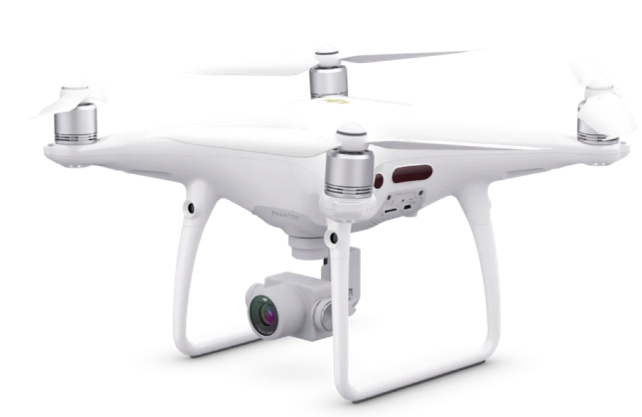
\includegraphics[width=\textwidth]{./api/phantom4.png}
        \caption{DJI Phantom 4}
        \label{fig:manifold}
    \end{subfigure}
    \caption{Présentation des UAV disponibles à l'ENSTA Bretagne}
    \label{fig:environnement}
\end{figure}

Le DJI Phantom 4 est un UAV grand public, utilisé pour faire de la vidéo. Son capteur
haut-de-gamme produit des images stables et de haute résolution. L’UAV est de plus
équipé de nombreux capteurs sur ses faces pour éviter des obstacles et se positionner.
Des algorithmes sont déjà embarqués sur le drone pour effectuer des missions plus ou
moins évoluées. Nous aimerions pouvoir contrôler l’UAV via un middleware comme
ROS. DJI propose deux pistes: un \textit{Windows SDK} et un Android SDK. Le \textit{Windows SDK}
a la contrainte de la programmation en C\#, de plus ROS est nativement développé pour
fonctionner sous Android. Nous avons donc retenu le \textit{Android SDK}, c’est une API
fonctionnant en Java le langage de programmation d’Android. Il existe une classe
appelée \texttt{virtualRemote} \footnote{\url{https://developer.dji.com/api-reference/android-api/Components/MobileRemoteController/DJIMobileRemoteController.html}} , permettant de commander l’UAV en poussées et angles
d’Euler grâce à des méthodes comme \texttt{setLeftStickVertical} ou \texttt{getRightStickHorizontal}  .

ROS propose un package fonctionnant sur Android. Toutes les briques sont présentes
pour ainsi connecter le ROS Master du PC au à la \texttt{virtualRemote} de l’API. L’architecture
électronique est présentée dans la figure \ref{fig:architecture}.

\begin{figure}[!htb]
    \centering
    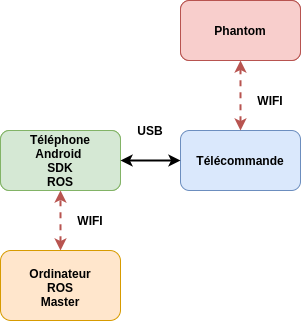
\includegraphics[width=0.4\textwidth]{./api/architecture.png}
    \caption{Architecture électronique.}
    \label{fig:architecture}
\end{figure}


En nous inspirant des exemples de DJI Developer, nous avons pu construire une
application permettant de contrôler le Phantom 4 avec des fonctions basiques.
Cependant nous n’avons pas fait la liaison avec ROS. En effet, nous attendions d’avoir
un contrôleur fonctionnant correctement en simulation avant d’automatiser le pilotage
du drone.

